In this section, we look into the basic summary and properties of different assets.

\subsection{Statistics}
Symbol explanation:

i: represents different index.

t: time period.

\begin{itemize}
\item Annualised return \\
Annualised return are calculated based on the daily returns. 
\begin{equation}
R_a = (1+R_d)^{N} -1
\end{equation}
where $R_a$ is the annualized returns, $R_d$ is the daily returns, N is the number of trading days in one year (N = 252).
\item Sharpe Ratio
\begin{equation}
sharpe\_ratio = \frac{\bar{r}_i-Rf}{\sigma_i}
\end{equation}
Here we let $Rf = 0$
\item Standard deviation
\begin{equation}
standard\_deviation_i =\sqrt{ \frac{1}{n-1}\sum_{t=1}^n{(r_i^t-\bar{r}_i)^2}} 
\end{equation}
\item Skewness
\begin{equation}
skewness_i = E_t \left[ \left( \frac{r_i^t-\bar{r}_i}{\sigma_i} \right)^3 \right]
\end{equation}
\item Kurtosis
\begin{equation}
kurtosis_i = \frac{E_t \left[ \left( r_i^t-\bar{r}_i \right)^4 \right]}{\left(E_t \left[ \left( r_i^t-\bar{r}_i \right)^2 \right]\right)^2}
\end{equation}
\end{itemize}

\subsection{Summary}

\subsubsection{Returns}

Figure \ref{fig: dailyReturns} shows the returns over time for each asset (calculated based on their individual time range). We can see an obvious increase in volatilities during financial crises such as Black Monday in 1987 and the great recession in 2008. While GO01 (which is treated as the risk free rate in our analysis) has the smallest return, RMZ has the highest return as well as a highest volatility. Figure \ref{fig: returnsDist} show the empirical distribution of daily returns for each asset. The Kolmogorov tests show that the returns do not follow normal distribution ($p < 10^{-5}$). And the asset returns have a fatter tails than normal distribution. This result is unsurprising since fat tail is a quite common phenomenon in asset returns. 

%%%%%%%
\iffalse

\begin{figure}[h]
\caption{Daily Returns} 
\centering 
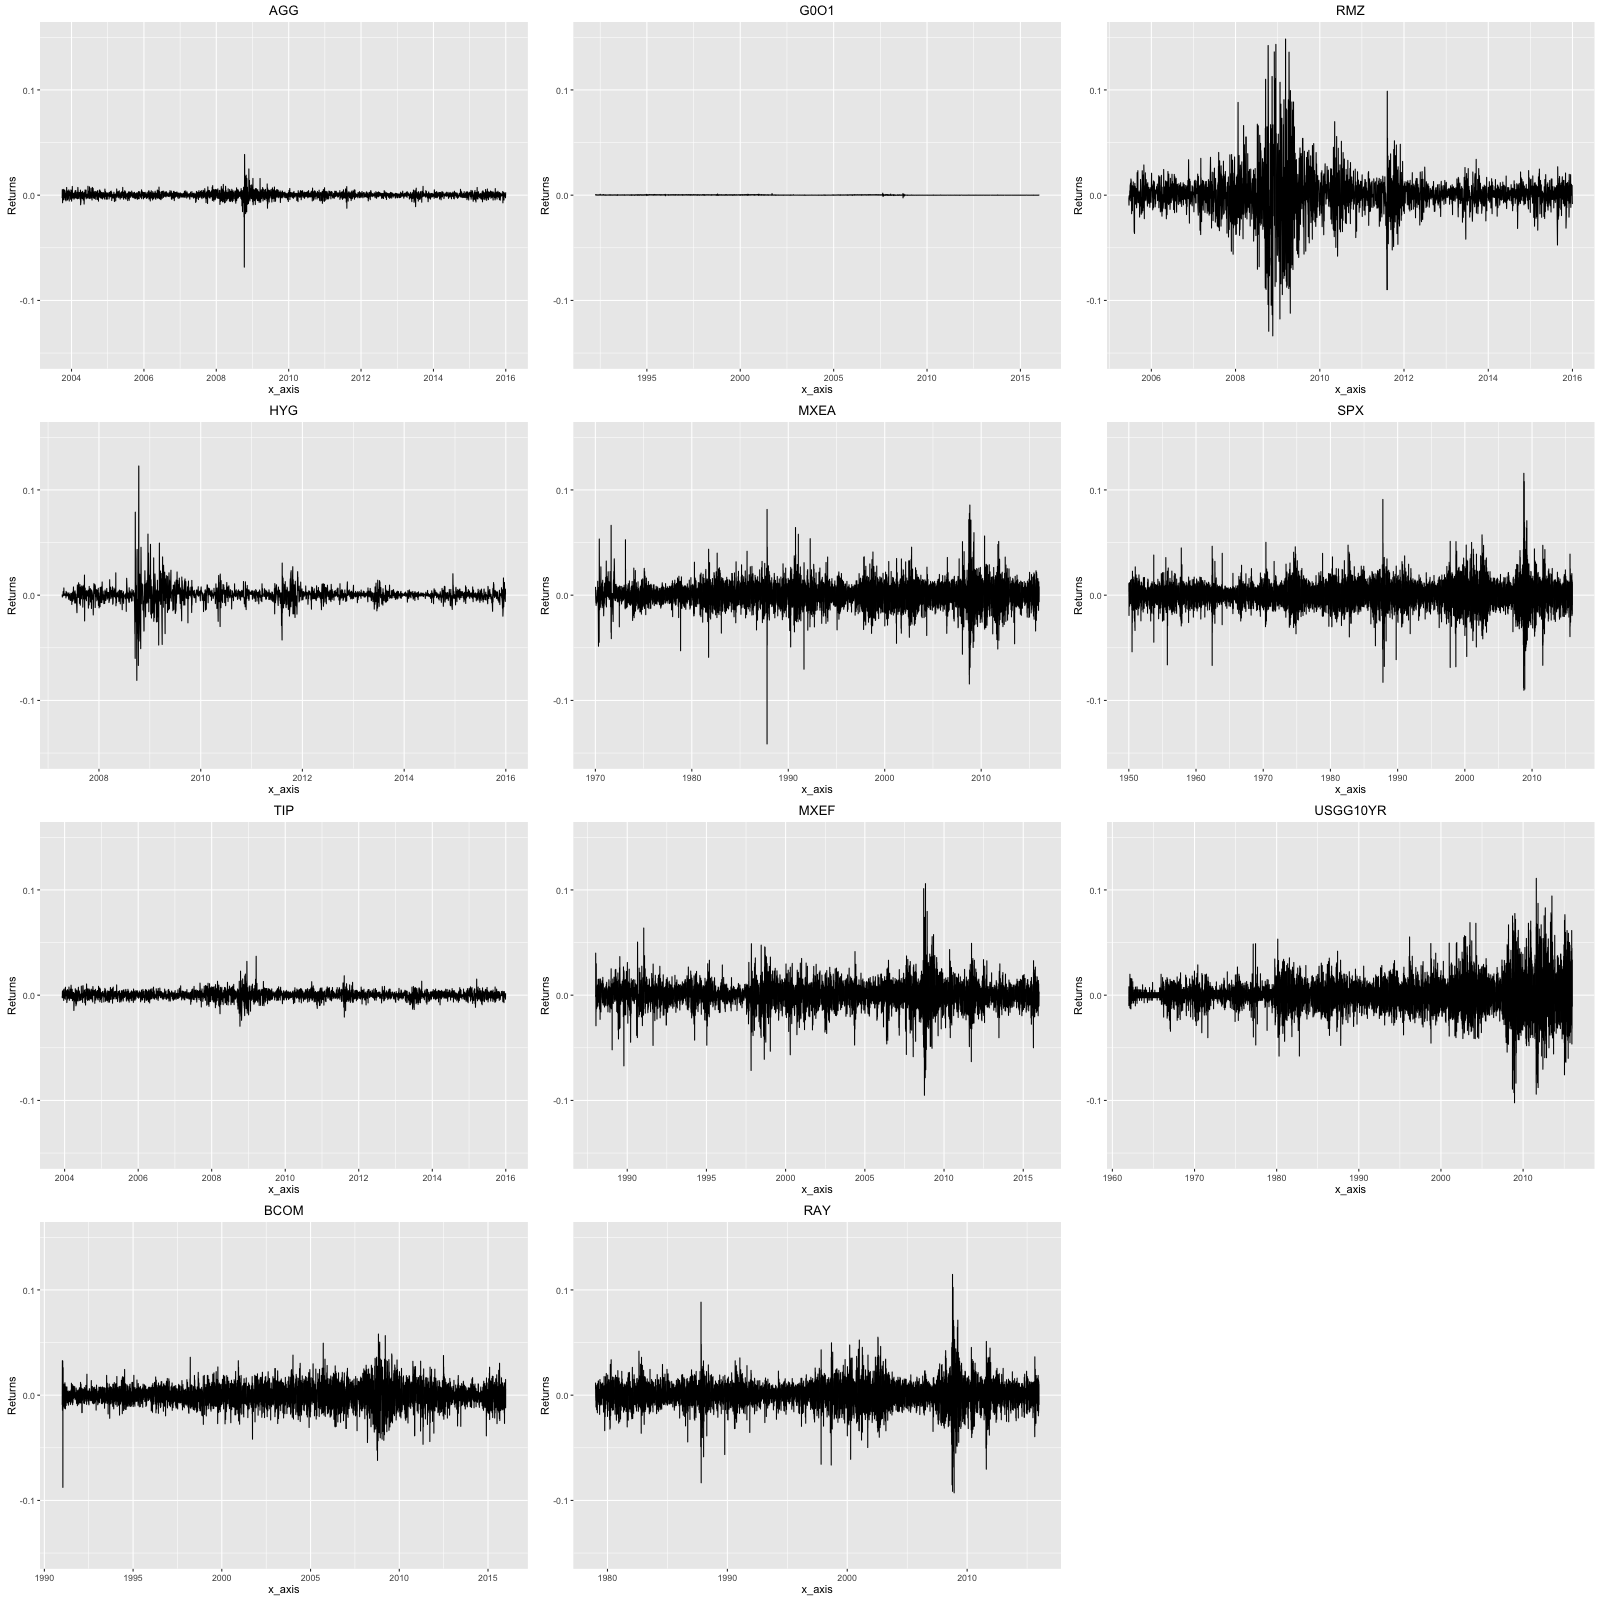
\includegraphics[width=15cm]{../results/returns}
\label{fig: dailyReturns}
\end{figure}

\begin{figure}[h]
\caption{Empirical distribution of daily returns} 
\centering 
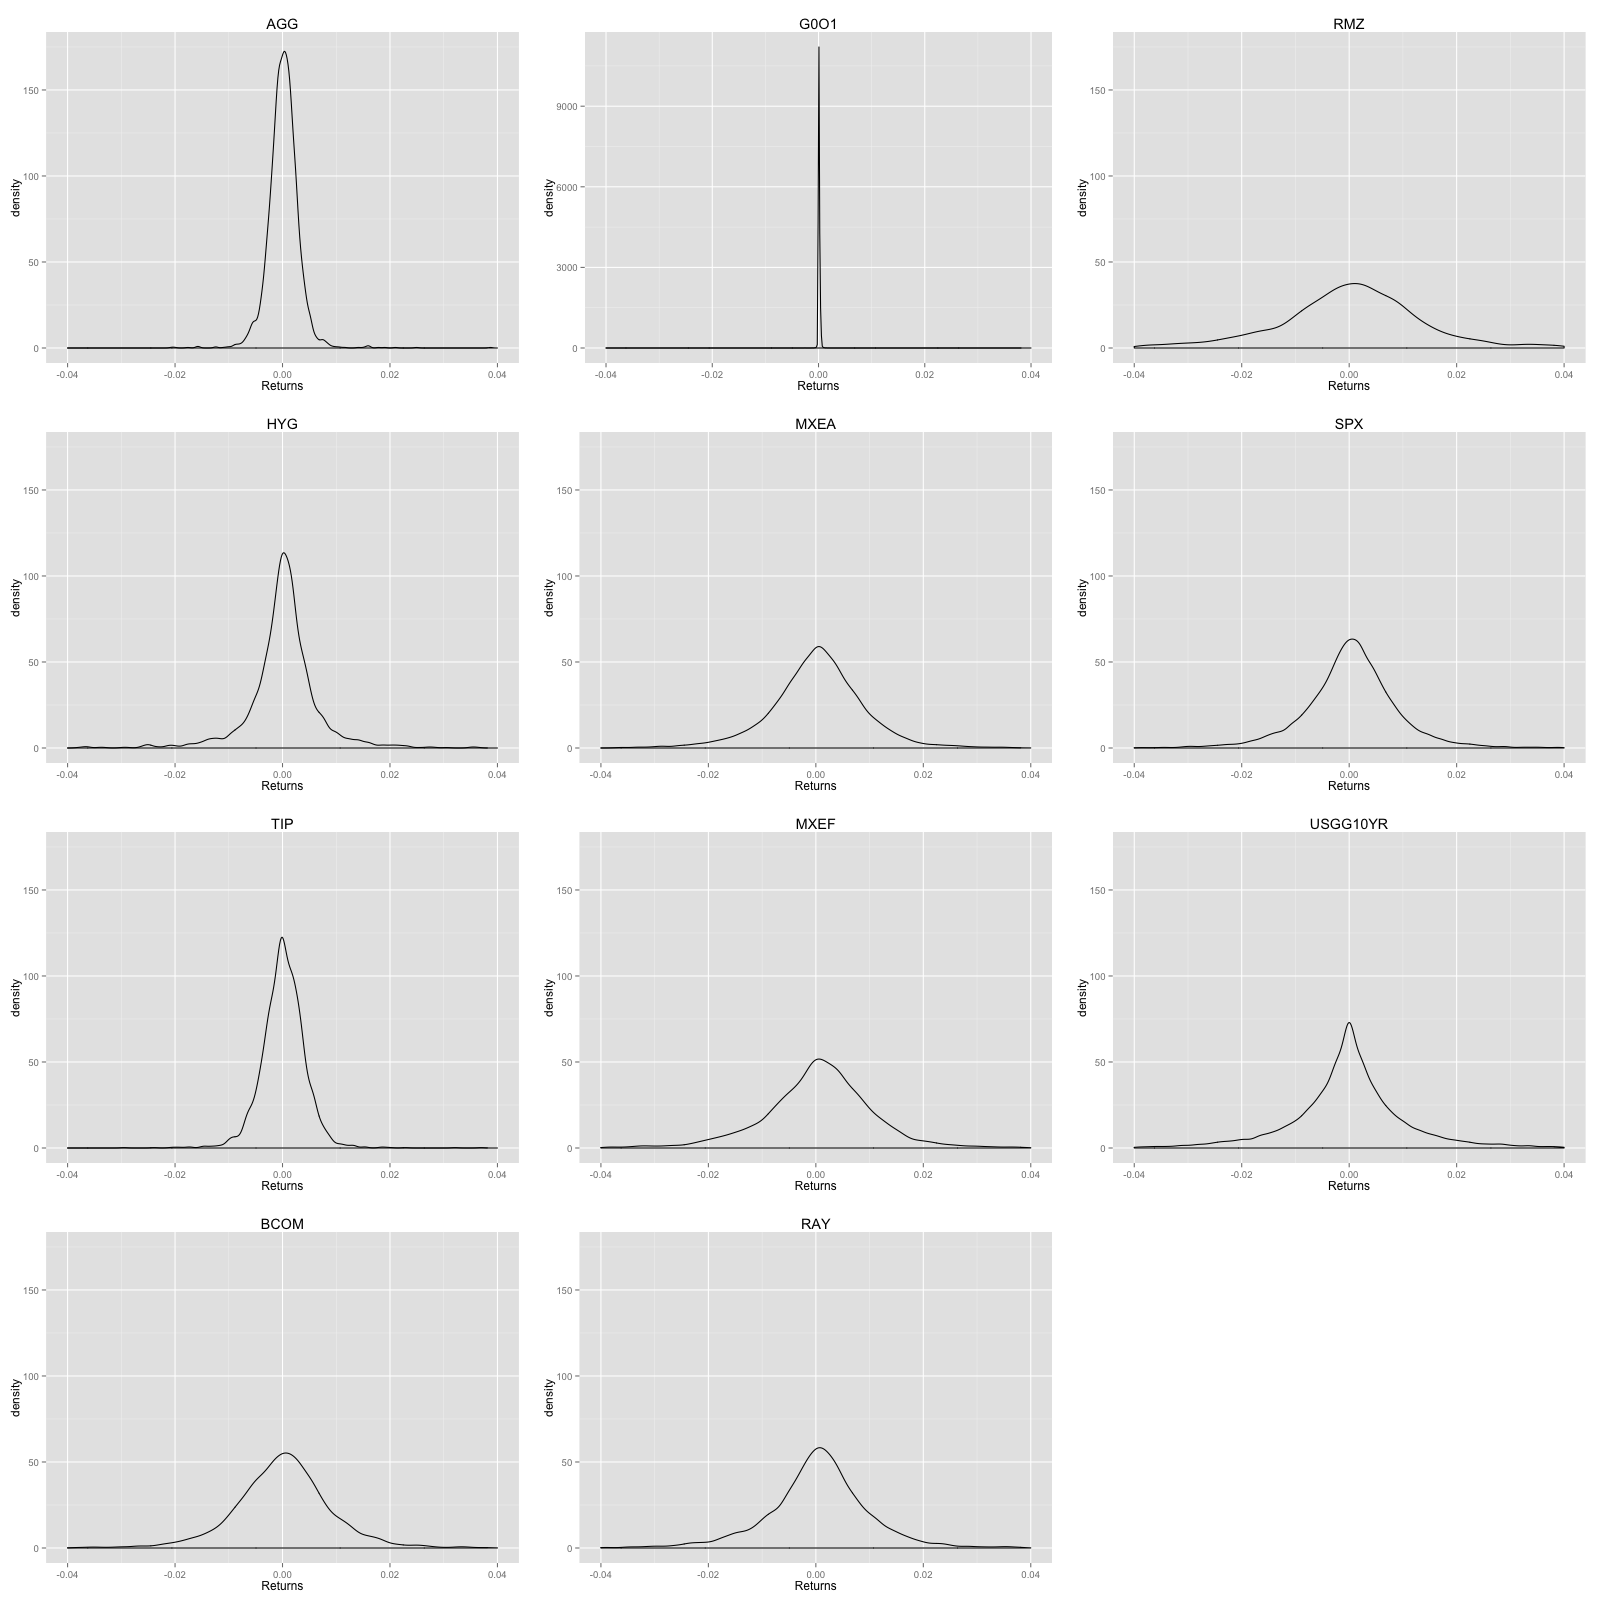
\includegraphics[width=15cm]{../results/returns_dist}
\label{fig: returnsDist}
\end{figure}

\fi
%%%%%%%%

\subsubsection{Statistical summary}

Table \ref{table:statSum} presents the statistical summary of each assets (calculated based on their individual time range). Note that here all asset returns have positive kurtosis (leptokurtic), and nonzero skewness (with both positive and negative values). This is consistent with the Kolmogorov test results in last subsection which show the asset return distribution generally have fat tails.

\begin{table}[!h]
\caption{Statistical Summary of Assets} 
\centering 
\begin{tabular}{ | c || p{1.5cm} p{1.2cm} r r | } 
 \hline
Asset & Sharpe  & Sd. & Skewness & Kurtosis \\
  \hline \hline
AGG & 0.052 & 0.051 & -2.51 & 81.31\\ 
HYG & 0.025 & 0.134 &  0.87 & 36.71\\ 
TIP & 0.040 & 0.065 &  0.10 &  6.48\\ 
BCOM & 0.001 & 0.149 & -0.27 &  4.33\\ 
G0O1 & & 0.002 &  0.69 & 26.76\\ 
MXEA & 0.030 & 0.155 & -0.32 & 10.74\\ 
MXEF & 0.031 & 0.180 & -0.39 &  7.71\\ 
RAY & 0.036 & 0.173 & -0.66 & 17.22\\ 
RMZ & 0.016 & 0.366 &  0.36 & 13.68\\ 
SPX & 0.035 & 0.153 & -0.65 & 21.12\\ 
USGG10YR & 0.003 & 0.201 &  0.12 &  8.81\\
 \hline
\end{tabular}
\label{table:statSum}
\end{table}